\documentclass[fleqn,pdf, 9pt, usenames, dvipsnames, unicode, hyperref={bookmarks=true,bookmarksopen=false, bookmarksnumbered}]{beamer}
\setbeamersize{text margin left=0.8in,text margin right=0.8in}
\usepackage[T2A,T1]{fontenc}
\usepackage[english,russian]{babel}
\usepackage[utf8]{inputenc}
\usepackage{graphicx}
\usepackage{amsmath,amssymb,amsthm}
% \usepackage{anyfontsize}
\usepackage{tcolorbox}
\usepackage{amsfonts}
\usepackage{ulem}
\usepackage{delarray}
\usepackage{multicol}
\usepackage{enumerate}
\usepackage{amsmath}
\usepackage[thinc]{esdiff}
\usepackage{mathtools}
\usepackage{breqn}
\graphicspath{{FIG/}}
\usefonttheme[onlymath]{serif}
\usepackage{beamerthemesplit}
\setbeamerfont{institute}{size=\normalsize}
\setbeamercolor{bluetext_color}{fg=blue}
\newcommand{\bluetext}[1]{{\usebeamercolor[fg]{bluetext_color}#1}}
\setbeamercovered{transparent}
\DeclareMathOperator{\sign}{sign}
\usepackage[update,prepend,suffix=]{epstopdf}
\newcommand{\alarm}[1]{\textcolor{red}{#1}}
\newcommand{\alarmg}[1]{\textcolor{blue}{#1}}
%%%%%%%%%%%%%%%%%%%%%%%%%%%%%%%%%%%%%%%%
% Изменение размеров footline
\defbeamertemplate*{footline}{my footline}{
  \leavevmode%
  \hbox{\begin{beamercolorbox}[wd=.2\paperwidth,ht=2.5ex,dp=1.125ex,leftskip=.3cm,rightskip=.3cm plus1fill]{author in head/foot}%
    \usebeamerfont{author in head/foot}\insertshortauthor
  \end{beamercolorbox}%
  \begin{beamercolorbox}[wd=.8\paperwidth,ht=2.5ex,dp=1.125ex,leftskip=.3cm,rightskip=.3cm plus1fil]{title in head/foot}%
    \usebeamerfont{title in head/foot}\insertshorttitle
  \end{beamercolorbox}}%
  \vskip0pt%
}\usebeamertemplate{my footline}
% Изменение размеров footline

% insert page numbers
\expandafter\def\expandafter\insertshorttitle\expandafter{%
  \insertshorttitle\hfill%
  \insertframenumber/\inserttotalframenumber}
% insert page numbers
\linespread{1.3}
%%%%%%%%%%%%%%%%%%%%%%%%%%%%%%%%%%%%%%%%
\setbeamercolor{bcgreen}{bg=green!100!black,fg=black}
\setbeamercolor{bcyellow}{bg=yellow!100!black,fg=black}
\setbeamercolor{bcred}{bg=red!100!black,fg=white}
\setbeamercolor{bcgray}{bg=white!80!black,fg=black}

\definecolor{anti-flashwhite}{rgb}{0.95, 0.95, 0.96}
\definecolor{blond}{rgb}{0.98, 0.94, 0.75}
\definecolor{brickred}{rgb}{0.8, 0.25, 0.33}

\title{Композиция методов}

\author[Леонович.Р.А]
{Леонович.Р.А}

\institute[shortinst]{Санкт-Петербургский государственный университет\\Прикладная математика и информатика\\ Кафедра Статистического Моделирования
}

\vspace{6mm}
\date{
	СПб, 2021\\[6mm]

}

\usepackage{cmap}

\begin{document}

%%%%%%%%%%%%%%%%%%%%%%%%%%%%%%%%%%%%%%%%%%%%%%%%%%%%
	
%%%%%%%%%%%%%%%%%%%%%%%%%%%%%%%%%%%%%%%%%%%%%%%%%%%%%%%%%%%%%%%%%%%%%%%%

\begin{frame}
\titlepage
\end{frame}

%%%%%%%%%%%%%%%%%%%%%%%%%%%%%%%%%%%%%%%%%%%%%%%%%%%%
	
\begin{frame}\frametitle{План}

\begin{enumerate}
    \item Bootstrap
    \item Разложение на смещение и разброс
    \item Bagging
    \item Random Forest
    \item Boosting
        \begin{enumerate}
            \item Градиентный бустинг
            \item Градиентный бустинг над деревьями
            \item Взвешивание объектов
        \end{enumerate}
\end{enumerate}

\end{frame}
	
%%%%%%%%%%%%%%%%%%%%%%%%%%%%%%%%%%%%%%%%%%%%%%%%%%%%
	
\begin{frame}\frametitle{Bootstrap}

\begin{itemize}
    \item Дано $\mathbf{X} \in \mathbb{R}^{n\times p}$ --- набор данных, $\mathbf{Y}\in \mathbb{R}^{n}$ --- зависимые переменные,    $X = (x_i,y_i)$. 
    \item Возьмем $l$ объектов с возвращениями --- $X_1$
    \item Повторим $N$ раз --- $X_1,\ldots,X_N$
    \item Обучим по каждой выборке модель линейной регрессии и получим базовые алгоритмы $b_1(x),\ldots,b_N(x)$
    \item Предположим, что существует модель $y(x) = \sum \beta_i x_i + \epsilon_i $ и $p(x)$ --- распределение  $\mathbf{X}$ .
    \item Ошибка регрессии: $\epsilon_j(x)=b_j(x)-y(x),\qquad j = 1,...,N.$
    \item $\mathbb{E}_x\epsilon^2_j(x) = \mathbb{E}_x\left(b_j(x) - y(x)\right)^2 $
\end{itemize}

\end{frame}

%%%%%%%%%%%%%%%%%%%%%%%%%%%%%%%%%%%%%%%%%%%%%%%%%%%%

\begin{frame}\frametitle{Среднеквадратичная ошибка}

Средняя ошибка построенных функций регрессии: 
$E_1 =  \dfrac{1}{N}\sum_{j=1}^{N}\mathbb{E}_x\epsilon^2_j(x)$

Пусть 
$\mathbb{E}_x\epsilon_j(x) = 0$ \qquad и \qquad
$ \mathbb{E}_x\epsilon_i(x)\epsilon_j(x) = 0$,  $i\neq j$

и $a(x) = \frac{1}{N}\sum_{j=1}^{N}b_j(x)$ 

Тогда 

$E_N = \mathbb{E}_x\left(\frac{1}{N}\sum_{j=1}^{N}b_j(x)-y(x)\right)^2 = \mathbb{E}_x\left(\frac{1}{N}\sum_{j=1}^{N}\epsilon_j(x)\right)^2 = $

$=\frac{1}{N^2}\mathbb{E}_x\left(\sum_{j=1}^{N}\epsilon^2_j(x) + \sum_{i\neq j}^{}\epsilon_i(x)\epsilon_j(x)\right)=\frac{1}{N}E_1$

\end{frame}

%%%%%%%%%%%%%%%%%%%%%%%%%%%%%%%%%%%%%%%%%%%%%%%%%%%%

\begin{frame}\frametitle{Разложение на смещение и разброс}


Пусть задана выборка $X = (x_i,y_i)^l_{i=1}$ с ответами $y_i \in \mathbb{R}$ и $\exists p(x,y)$

Рассмотрим $L(y,a) = (y-a(x))^2$ --- функция потерь,

и $R(a) = \mathbb{E}_{x,y}\left[(y-a(x))^2\right] \int_{\mathbb{X}}\int_{\mathbb{Y}} p(x,y)(y-a(x))^2dxdy$ --- ее среднеквадратичный риск.

\end{frame}

%%%%%%%%%%%%%%%%%%%%%%%%%%%%%%%%%%%%%%%%%%%%%%%%%%%%

\begin{frame}\frametitle{Ошибка метода обучения}

Метод обучения: $\mu : (\mathbb{X}\times\mathbb{Y})^l \rightarrow \mathbf{A}$

\begin{equation}
\begin{split}
	&L(\mu) = \mathbb{E}_X\left[\mathbb{E}_{x,y}\left[ \left(y-\mu(X)(x))\right)^2\right]\right] =  \\ &=\int_{(\mathbb{X}\times\mathbb{Y})^l}\int_{\mathbb{X}\times\mathbb{Y}} \left(y-\mu(X)(x)\right)^2 p(x,y) \times \\ &\times \prod^l_{i=1}p(x_i,y_i)dxdydx_1dy_1,\ldots dx_ldy_l
	\label{risk}
	\end{split}
\end{equation}

Здесь, $\mathbb{E}_X[\cdot]$ берется по всем возможным выборкам ${(x_1, y_1), . . . ,(x_l, y_l)}$
из распределения $\prod_{i=1}^{l}p(x_i,y_i)$

$\mathbb{E}_{x,y} = \left[(y-\mu(X))^2\right] = \mathbb{E}_{x,y}\left[(y-\mathbb{E}[y|x])^2\right] + \mathbb{E}_{x,y}\left[(\mathbb{E}[y|x] - \mu(X))^2\right]$ ---

Среднеквадратичный риск на фиксированной выборке $X$

Подставим это в формулу (\ref {risk})

\end{frame}

%%%%%%%%%%%%%%%%%%%%%%%%%%%%%%%%%%%%%%%%%%%%%%%%%%%%

\begin{frame}\frametitle{Ошибка метода обучения (продолжение)}

\begin{equation}
	\begin{split}
	&L(\mu) = \mathbb{E}_X\left[\underbrace{\mathbb{E}_{x,y}\left[(y-\mathbb{E}[y|x])^2\right]}_{\text{не завсисит от X}} + \mathbb{E}_{x,y}\left[(\mathbb{E}[y|x] - \mu(X))^2\right]\right] = \\
	&= \mathbb{E}_{x,y}\left[(y-\mathbb{E}[y|x])^2\right] + \mathbb{E}_{x,y}\left[\mathbb{E}_X \left[(\mathbb{E}[y|x]- \mu(X))^2\right]\right]
\end{split}
\label{2.2}
\end{equation}

Преобразовываем второе слагаемое:
\begin{equation}
    \begin{aligned}
        &\mathbb{E}_{x,y}\left[\mathbb{E}_X \left[(\mathbb{E}[y|x] - \mu(X))^2\right]\right] = \\ 
        &= \mathbb{E}_{x,y}\left[\mathbb{E}_X \left[(\mathbb{E}[y|x] - \mathbb{E}_X[\mu(X)] + \mathbb{E}_X[\mu(X)] -\mu(X))^2\right]\right] = \\
        &=
	\mathbb{E}_{x,y}\left[\mathbb{E}_X \left[\underbrace{(\mathbb{E}[y|x] - \mathbb{E}_X \mu(X))^2}_{\text{не завсисит от X}}\right]\right] + \mathbb{E}_{x,y}\left[\mathbb{E}_X \left[(\mathbb{E}_X \mu(X) - \mu(X))^2\right]\right] + \\ 
	&+ 
	2\mathbb{E}_{x,y} \left[\mathbb{E}_X\left[(\mathbb{E}[y|x] - \mathbb{E}_X[\mu(X)])(\mathbb{E}_X[\mu(X)]-\mu(X))\right]\right]
	\label{2.3}
    \end{aligned}
\end{equation}



\end{frame}

%%%%%%%%%%%%%%%%%%%%%%%%%%%%%%%%%%%%%%%%%%%%%%%%%%%%

\begin{frame}\frametitle{Ошибка метода обучения (продолжение)}

    Подставим (\ref{2.3}) в (\ref{2.2}).
    \begin{gather}
	L(\mu) = \underbrace{\mathbb{E}_{x,y}\left[(y-\mathbb{E}[y|x]^2)\right]}_{\text{шум}} + \\ +
	\underbrace{\mathbb{E}_x\left[\mathbb{E}_X[\mu(X)] - \mathbb{E}[y|x]\right]}_{\text{смещение}} + \underbrace{\mathbb{E}_x\left[\mathbb{E}_X\left[(\mu(X) - \mathbb{E}_X[\mu(X)])^2\right]\right]}_{\text{разброс}}
	\label{2.4}
\end{gather}


\end{frame}

%%%%%%%%%%%%%%%%%%%%%%%%%%%%%%%%%%%%%%%%%%%%%%%%%%%%

\begin{frame}\frametitle{Пример}

\begin{figure}[!ht]
	\centering
	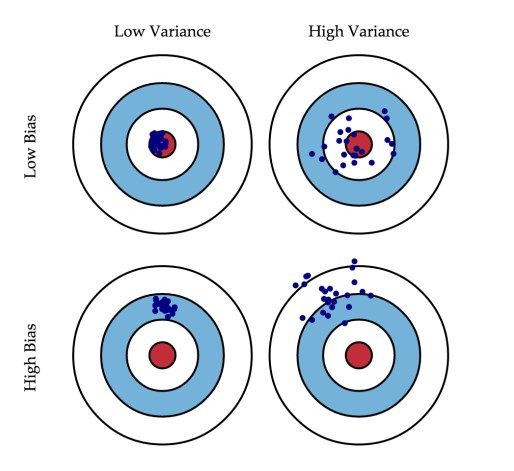
\includegraphics[width=0.7\textwidth]{bias_var.jpg}
	\caption{Сдвиг и разброс разных моделей}
	\label{fig:bias_var}
\end{figure}

\end{frame}

%%%%%%%%%%%%%%%%%%%%%%%%%%%%%%%%%%%%%%%%%%%%%%%%%%%%

\begin{frame}\frametitle{Bagging}

Возьмем некоторый метод обучения $\mu(X)$. Построим на его основе метод $\hat{\mu}(X)$, который гененирует случайную подвыборку $\hat{X}$ с помощью бутстрапа и подает ее на вход метода $\mu: \hat{\mu}(X) = \mu(\hat{X})$

\begin{equation}
	{a}_{N}(x) = \dfrac{1}{N}\sum_{n=1}^{N}b_n(x) = \dfrac{1}{N}\sum_{n=1}^{N}\hat{\mu}(x)
\end{equation}

\end{frame}

%%%%%%%%%%%%%%%%%%%%%%%%%%%%%%%%%%%%%%%%%%%%%%%%%%%%

\begin{frame}\frametitle{Смещение и разброс для бэггинга}

Из (\ref{2.4}), смещение будет равно:

\begin{multline}
	\mathbb{E}_{x,y}\left[\left(\mathbb{E}_X\left[\frac{1}{N}\sum_{b=1}^{N}\hat{\mu}(X)(x)\right]-\mathbb{E}[y|x]\right)^2\right] = \\ = \mathbb{E}_{x,y}\left[\left(\frac{1}{N}\sum_{b=1}^{N}\mathbb{E}_X\hat{\mu}(X)(x)\right)\right]  =\mathbb{E}_{x,y}\left[(\mathbb{E}_X\left[\hat{\mu}(X)(x)\right]-\mathbb{E}[y|x])^2\right]
\end{multline}

Разброс: 

\begin{multline}
	\frac{1}{N}\mathbb{E}_{x,y}\left[\mathbb{E}_X\left[\left(\hat{\mu}(X)(x)-\mathbb{E}_X[\hat{\mu}(X)(x)]\right)^2\right]\right] + \\ + 
	\frac{N(N-1)}{N^2}\mathbb{E}_{x,y}[\mathbb{E}_X[\left(\hat{\mu}(X)(x)-\mathbb{E}_X[\hat{\mu}(X)(x)]\right)\times \\ \times \left(\hat{\mu}(X)(x)-\mathbb{E}_X[\hat{\mu}(X)(x)]\right)]]
\end{multline}


\end{frame}

%%%%%%%%%%%%%%%%%%%%%%%%%%%%%%%%%%%%%%%%%%%%%%%%%%%%

\begin{frame}\frametitle{Out-of-Bag Error Estimation}

$OOB = \sum_{i=1}^{l}L\left(y_i,\frac{1}{\sum_{n=1}^{N}\left[x_i \notin X_n\right]}\sum_{n=1}^{N}[x_i\notin X_n]b_n(x_i)\right)$

\end{frame}

%%%%%%%%%%%%%%%%%%%%%%%%%%%%%%%%%%%%%%%%%%%%%%%%%%%%

\begin{frame}\frametitle{Random Forest}

\textbf{Алгоритм:}
Для $n=1,\ldots,N$
\begin{enumerate}
	\item Сгенерировать выборку $\hat{X}_n$ с помощью бутстрапа.
	\item Построить решающее дерево $b_n(x)$ по выборке $\hat{X}_n$.
	\begin{itemize}
		\item дерево строится, пока в каждом листе не окажется не более $n_{min}$ объектов
		\item при каждом разбиении сначала выбирается $m$ случайных признаков из $p$ и оптимальное разделение ищется только среди них
	\end{itemize}
	\item Вернуть композицию $a_N(x) = \dfrac{1}{N}\sum_{n=1}^{N}b_n(x)$
\end{enumerate}

В случайных лесах признак, по которому производится разбиение, выбирается из их случайного подмножества размера $m$.

Рекомендуется в задачах классификации брать $m=\sqrt{p}$, а в задачах регрессии --- $m=p/3$

\end{frame}

\begin{frame}\frametitle{Сравнение бэггинга и случайного леса}

\begin{figure}[!ht]
	\centering
	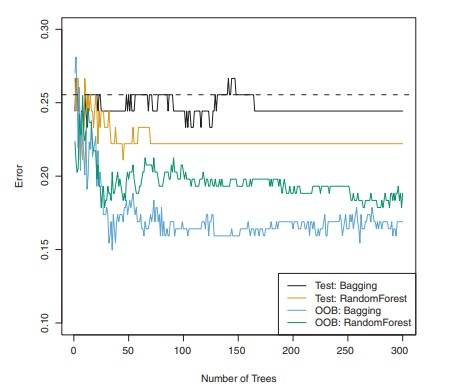
\includegraphics[width=0.8\textwidth]{bag_rf.jpg}
	\caption{График изменения ошибки моделей}
	\label{fig:bias_var}
\end{figure}

\end{frame}

%%%%%%%%%%%%%%%%%%%%%%%%%%%%%%%%%%%%%%%%%%%%%%%%%%%%

\begin{frame}\frametitle{Бустинг в задаче регрессии}

Минимизация квадратичного функционала:

$\dfrac{1}{2}\sum_{i=1}^{l}(a(x_i)-y_i)^2 \rightarrow \underset{a}{min}$

Будем искать итоговый алгоритм в виде суммы базовых моделей $b_n(x)$:

$a_N(x) = \sum_{n=1}^{N}b_n(x)$, где базовые алгоритмы $b_n \in \mathbf{A}$.

Первый базовый алгоритм: $b_1(x):= \underset{b\in\mathbf{A}}{argmin} \dfrac{1}{2}\sum_{i=1}^{l}(b(x_i)-y_i)^2$.

Остатки на каждом объекте:  $s^{(1)}_i = y_i - b_i(x)$

$b_2(x) := \underset{b\in\mathbf{A}}{argmin} \dfrac{1}{2}\sum_{i=1}^{l}(b(x_i)-s^{(1)})^2$



\end{frame}

%%%%%%%%%%%%%%%%%%%%%%%%%%%%%%%%%%%%%%%%%%%%%%%%%%%%

\begin{frame}\frametitle{Бустинг в задаче регрессии (продолжение)}

Таким образом, каждый следующий алгоритм тоже будем настраивать на остатки предыдущих:

$s^{(N)}_i = y_i - \sum_{n=1}{N-1}b_n(x_i) = y_i - a_{N-1}(x_i)$,

$i=1,\ldots,l$

$b_N(x):= \underset{b\in\mathbf{A}}{argmin} \dfrac{1}{2}\sum_{i=1}^{l}(b(x_i)-s_i^{(N)})^2$

Также, остатки могут быть найдены как антиградиент функции потерь по ответу модели, посчитанный в точке ответа уже построенной композиции:

$s_i^{(N)} = y_i - a_{N-1}(x_i)= \left.- \diff{p}{z}\dfrac{1}{2}(z-y_i)^2\right|_{z=a_{N-1}(x_i)}$

\end{frame}

%%%%%%%%%%%%%%%%%%%%%%%%%%%%%%%%%%%%%%%%%%%%%%%%%%%%

\begin{frame}\frametitle{Градиентный бустинг}

Пусть дана некоторая дифференцируемая функция потерь $L(y, z)$. 

Будем строить взвешенную сумму базовых алгоритмов:
$a_N(x) = \sum_{n=0}^{N}\gamma_n b_n(x)$

\textbf{Примеры выбора алгоритма $b_0(x)$:}

\begin{enumerate}
	\item Нулевой: $b_0(x) = 0$.
	\item Возвращающий самый популярный класс (в задачах классификации):
	
	$b_0(x) = \underset{y\in\mathbf{\mathbb{Y}}}{argmax}\sum_{i=1}^{l}[y_i=y]$
	\item Возвращающий средний ответ (в задачах регрессии):	
	$b_0(x) = \frac{1}{l}\sum_{i=1}{l}y_i$
\end{enumerate}

\end{frame}

%%%%%%%%%%%%%%%%%%%%%%%%%%%%%%%%%%%%%%%%%%%%%%%%%%%%

\begin{frame}\frametitle{Градиентный бустинг (продолжение)}

Допустим, мы построили композицию $a_{N-1}(x)$ из $N-1$ алгоритма, и хотим выбрать следующий абзовый алгоритм $b_N(x)$ так, чтобы как можно сильнее уменьшить ошибку:

$\sum_{i=1}^{l} L\left(y_i,a_{N-1}(x_i) + \gamma_N b_N(x_i)\right)\rightarrow \underset{b_N,\gamma_N}{min}$

Какие числа $s_1,\ldots, s_l$ надо выбрать для решения следующей задачи:

$\sum_{i=1}^{l} L\left(y_i, a_{N-1}(x_i) +s_i\right)\rightarrow \underset{s_1,\ldots, s_l}{min}$

\end{frame}

%%%%%%%%%%%%%%%%%%%%%%%%%%%%%%%%%%%%%%%%%%%%%%%%%%%%

\begin{frame}\frametitle{Функция алгоритма}

\begin{itemize}
    \item    $s_i = y_i - a_{N-1}(x_i)$ \textbf{?}
    \item    $s_i = - \left. \diffp{L}{z} \right|_{z=a_{N-1}(x_i)}$
    
    В этом случае сдвиг $s_i$ будет противоположен производной функции потерь в точке $z=a_{N-1}(x_i)$:
     
    
\end{itemize}

Заметим, что вектор сдвигов $s = s_1,\ldots, s_l$ совпадает с антиградиентом:

$\left(\left. -\diffp{L}{z}\right|_{z=a_{N-1}(x_i)}\right)^l_{i=1} = -\bigtriangledown_z \sum_{i=1}^{l}\left. L(y_i,z_i) \right|_{z=a_{N-1}(x_i)}$

\end{frame}

%%%%%%%%%%%%%%%%%%%%%%%%%%%%%%%%%%%%%%%%%%%%%%%%%%%%

\begin{frame}\frametitle{Функция алгоритма (продолжение)}

По данным значениям в конечном числе точек необходимо построить функцию, заданную на всем пространстве объектов.

$b_N(x) = \underset{b\in\mathbf{A}}{argmin}\sum_{i=1}^{l} (b(x_i) - s_i)^2$ --- среднеквадратичная ошибка

$\gamma_N = \underset{\gamma\in\mathbf{\mathbb{R}}}{argmin}\sum_{i=1}^{l} L(y_i,a_{N-1}(x_i) + \gamma b_N(x_i))$ --- подбор коэффициента

\end{frame}

%%%%%%%%%%%%%%%%%%%%%%%%%%%%%%%%%%%%%%%%%%%%%%%%%%%%

\begin{frame}\frametitle{Регуляризация}

\begin{itemize}
    \item Сокращение шага
    
    $a_N(x) = a_{N-1}(x) + \eta\gamma_Nb_N(x)$, где $\eta \in (0,1]$ --- темп обучения.
    \item Стохастический градиентный бустинг
    
    
    
\end{itemize}

\end{frame}

%%%%%%%%%%%%%%%%%%%%%%%%%%%%%%%%%%%%%%%%%%%%%%%%%%%%

\begin{frame}\frametitle{Функции потерь}

\begin{itemize}
    \item Регрессия
    
    \begin{itemize}
        \item Квадратичная $\sum_{i=1}^{l}(a(x_i)-y_i)^2 \rightarrow \underset{a}{min}$
        \item Модуль отклонения $L(y,z) = |y-z|$, для которого антиградиент вычисляется по формуле 

        $s_i^{(N)} = -sign(a_{N-1}(x_i)-y_i)$
    \end{itemize}
    
    \item Классификация
    
    $L(y,z) = log(1+exp(-yz))$
\newline
    Задача поиска базового алгоритма с ней принимает вид

    $b_N = \underset{b\in\mathbf{A}}{argmin}\sum_{i=1}^{l} (b(x_i) - \frac{y_i}{1+exp(y_ia_{N-1}(x_i))})^2$
\end{itemize}


\end{frame}

%%%%%%%%%%%%%%%%%%%%%%%%%%%%%%%%%%%%%%%%%%%%%%%%%%%%

\begin{frame}\frametitle{Особенность логистической функции}

Ошибка на $N$-ой итерации:

$Q(a_N) = \sum_{i=1}^{l}log(1+exp(-y_ia_N(x_i))) = \sum_{i=1}^{l}log(1+exp(-y_ia_{N-1}(x_i))exp(-y_i \gamma_n b_N(x_i)))$

\hfill \break

Таким образом, величина $w_i^{(N)} = exp(-y_ia_{N-1}x(i))$ может случить мерой важности объекта $x_i$ на $N$-й итерации градиентного бустинга.

\end{frame}

%%%%%%%%%%%%%%%%%%%%%%%%%%%%%%%%%%%%%%%%%%%%%%%%%%%%

\begin{frame}\frametitle{Градиентный бустинг над деревьями}

$b_n(x) = \sum_{j=1}^{J_n} b_{nj}[x\in R_j]$, 

где $j=1,\ldots,J_n$ --- индексы листьев, $R_{j}$ --- соответствующие области разбиения, $b_{nj}$ --- значения в листьях.
\hfill \break

В $N$-й итерации бустинга композиция обновляется как

$a_N(x) = a_{N-1}(x) + \gamma_N \sum_{j=1}^{J_N}b_{Nj}[x\in R_j]$

\hfill \break

Можно улучшить качество композиции:
$\sum_{i=1}^{l} L\left(y_i,a_{N-1}(x_i) + \sum_{j=1}^{J_N} \gamma_{Nj}[x\in R_j]\right) \rightarrow \underset{\left\{\gamma_{Nj}\right\}^{J_N}_{j=1}}{min}$

\end{frame}

\begin{frame}\frametitle{Градиентный бустинг над деревьями (продолжение)}

Так как области разбиения $R_j$ не пересекаются, данная задача распадается на $J_N$ независимых подзадач:

$\gamma_{Nj} = \underset{\gamma}{argmin} \sum_{x_i \in R_j} L(y_i, a_{N-1}(x_i) + \gamma), \qquad j=1,\ldots, J_N$

\hfill \break

Логистическая функция потерь.

$F_j^{(N)}(\gamma) = \sum_{x_i \in R_j} log(1 + exp(-y_i(a_{N-1}(x_i) + \gamma))) \rightarrow \underset{\gamma}{min}$.

\end{frame}

\begin{frame}\frametitle{Смещение и разброс}

В случайных лесах:
\begin{itemize}
    \item Используются глубокие деревья, поскольку от базовых алгоритмов требуется низкое смещение.
    \item Разброс  устраняется за счёт усреднения ответов различных деревьев.
\end{itemize}

В бустинге:

\begin{itemize}
    \item Каждый следующий алгоритм понижает ошибку композиции.
    \item Переобучение при большом количестве базовых моделей.
    \item Можно понизить смещение моделей, а разброс либо останется таким же, либо увеличится.
    \item Используются неглубокие решающие деревья.
\end{itemize}


\end{frame}

\begin{frame}\frametitle{Сравнение случайного леса и бустинга}

\begin{figure}[!ht]
	\centering
	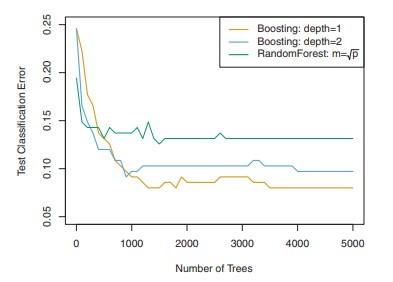
\includegraphics[width=0.8\textwidth]{rf_boost.jpg}
	\caption{График изменения ошибки моделей}
	\label{fig:rf}
\end{figure}

\end{frame}

\begin{frame}\frametitle{Взвешивание объектов}

AdaBoost: $L(y,z)= exp(-yz)$

\hfill \break

$L(a,X) = \sum_{i=1}^{l} exp\left(-y_i\sum_{n=1}^{N}\gamma_nb_n(x_i)\right)$

\hfill \break

Компоненты ее антиградиента после $N-1$ итерации:

$s_i=\left. -\diffp{L(y_i,z)}{z}\right|_z=a_{N-1}(x_i)$ $=y_i\underbrace{exp\left(-y_i\sum_{n=1}^{N-1}\gamma_nb_n(x_i)\right)}_{w_i}$


\end{frame}

\begin{frame}\frametitle{Влияние шума на обучение}

Рассмотрим теперь логистическую функцию потерь, которая также может использоваться в задачах классификации:

$L(a,X^l) = \sum_{i=1}^{l}log(1+exp(-y_ia(x_i)))$

\hfill \break

Ее антиградиент после $N-1$ шага:

$s_i = y_i \underbrace{\frac{1}{1+exp(y_ia_{N-1}(x_i))}}_{w_i^{(N)}}$


\end{frame}

% \begin{tcolorbox}[width=4.8in,left=0mm,right=0mm,top=0mm,bottom=0mm,boxrule=0pt]
% \begin{tcolorbox}[width=4.8in,left=0mm,right=0mm,top=0mm,bottom=0mm,colback=orange!50!white,boxrule=0pt] 
% \begin{tcolorbox}[width=4.8in,left=0mm,right=0mm,top=0mm,bottom=0mm,colback=Yellow!70!white,boxrule=0pt]

\end{document}